% ==================== Header ====================
\documentclass[12pt]{article} %montserrat fonts exists only in 10pt-12pt
\usepackage[a4paper, top=8mm, bottom=8mm, left=8mm, right=8mm]{geometry}
\usepackage[most]{tcolorbox}
\usepackage[hidelinks]{hyperref}
\usepackage{erewhon}
\usepackage[T2A]{fontenc} %For Cyrrylic
\usepackage[utf8]{inputenc} %For Cyrrylic
\usepackage{enumitem}
\usepackage{dirtytalk}
\usepackage{fontawesome5}
\usepackage{setspace}

\begin{document}

% ==================== Global settings ====================
\setlength{\parindent}{0mm} % No paragraph indent
\pagenumbering{gobble} % No page numbering

% ==================== Custom commands ====================
\definecolor{custom_blue}{RGB}{2,132,199}

\definecolor{linkedin_blue}{RGB}{10,102,194}

\newcommand{\NameText}[1] {{\Large\textbf{#1}}}

\newcommand{\HighlightedText}[1] {{\textbf{#1}}}

\newcommand{\PlaceAndTime}[2] {\HighlightedText{#1} \hfill \HighlightedText{#2}}

\newcommand{\SymbolAndLink}[3] {#1 \hspace{0mm} \href{#3} {\underline{#2}}}

\newcommand{\SymbolAndText}[2] {#1 \hspace{0mm} #2}

\newenvironment{ItemizeSection}[1]{
    \HighlightedText{#1}
    \vspace{1mm}
    {\color{custom_blue} \hrule}
    \begin{itemize}[topsep=0pt, itemsep=0pt, label={$\bullet$}]
}{
    \end{itemize}
}

\newenvironment{TextSection}[1]{
    \HighlightedText{#1}
    \vspace{1mm}
    {\color{custom_blue} \hrule}
    \begin{itemize}[topsep=0pt, itemsep=0pt, label={}]
}{
    \end{itemize}
}

\newenvironment{ItemizeSubsection}{
    \begin{itemize}[topsep=-999pt, itemsep=0pt, label={$\circ$}]
}{
    \end{itemize}
}

% ==================== Name and Contact ====================

\setstretch{1.1} % Spacing for thr header
\begin{tcolorbox}[sharp corners=all, colback=custom_blue, coltext=white, frame empty, left=2mm, right=2mm, top=1mm, bottom=1mm]

    \noindent \begin{minipage}{0.7\textwidth}
        \NameText{Кирило Совайло}

        \SymbolAndLink{\faAt}{k.sovailo@gmail.com}{mailto:k.sovailo@gmail.com}

        \SymbolAndLink{\faPhone*}{01763 5479038}{tel:+4917635479038}

        \SymbolAndLink{\faGithub}{github.com}{https://github.com/kyrylo-sovailo}

        \SymbolAndLink{\faLinkedin}{linkedin.com}{https://linkedin.com/in/kyrylo-sovailo-19b4541b9}

        \SymbolAndText{\faEnvelope}{Pallaswiesenstr. 39, 64293 Darmstadt}
    \end{minipage}
    \begin{minipage}{0.29\textwidth}
        \raggedleft
        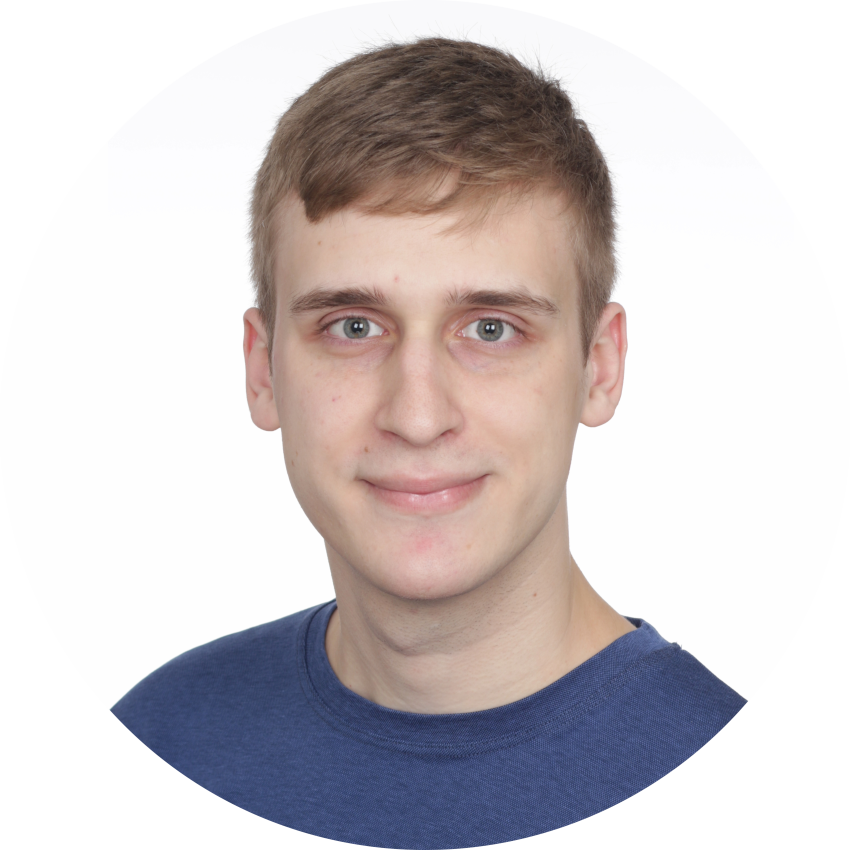
\includegraphics[width=35mm]{Photo_compressed_round.png}
    \end{minipage}
\end{tcolorbox}
\setstretch{1.0} % Spacing for the rest of the document

% ==================== Education ====================
\begin{ItemizeSection}{Освіта}
    \item \PlaceAndTime{Дармштадтський технічний університет}{2023 -- 2025} \\
    Computational Engineering, магістр

    \item \PlaceAndTime{Рейнсько-Вестфальський технічний університет Аахена}{2018 -- 2023} \\
    Computational Engineering Science, бакалавр

    \item \PlaceAndTime{Штудіенколлег при вільному університеті Берліна}{2017 -- 2018} \\
    Технічний курс (Т-курс)

    \item \PlaceAndTime{Технічний ліцей}{2010 -- 2017} \\
    Технічний Ліцей Національного Технічного Університету України \say{Київський Політехнічний Інститут}
\end{ItemizeSection}

% ==================== Professional background ====================
\begin{ItemizeSection}{Досвід}
    \item \PlaceAndTime{Магістерська робота в SIM при дармштадтському технічному університеті}{лютий -- вересень 2025}
    \begin{ItemizeSubsection}
        \item Title: Adding spatial awareness to embedding-based anomaly detection methods for automated industrial inspection
        \item Developed an anomaly detection method with >95\% accuracy by combining classic algorithms with foundation models (Python, torch, transformers)
    \end{ItemizeSubsection}

    \item \PlaceAndTime{Assistant at BMLS of Goethe University Frankfurt}{June 2023 -- July 2024}
    \begin{ItemizeSubsection}
        \item Developed graphical slicing software with support of features unique to a bio-3D-printer (C\#, C++, Slic3r)
        \item Ported printer control software to a new hardware (C++, Arduino)
    \end{ItemizeSubsection}

    \item \PlaceAndTime{Bachelor thesis at DSME of RWTH Aachen}{June -- September 2022}
    \begin{ItemizeSubsection}
        \item Title: Balancing a 2D inverted pendulum with a Franka Panda robotic arm
        \item Developed inverse kinematics, inverse dynamics, and control algorithms that enabled the robot to balance a 2-DOF inverse pendulum (ROS, C++, Python)
    \end{ItemizeSubsection}

    \item \PlaceAndTime{Intern at Continental AG}{March 2022 -- May 2022}
    \begin{ItemizeSubsection}
        \item Developed a tool for generation of C code from CAN database (Python, C, CAPL)
        \item Automated software building process for a V850 microcontroller (CMake, Python)
    \end{ItemizeSubsection}

    \item \PlaceAndTime{Assistant at DSME of RWTH Aachen}{April -- December 2021}
    \begin{ItemizeSubsection}
        \item Implemented high-level APIs and developed control algorithms for a Franka Panda robotic arm (real-time Linux, C++, Python)
        \item Implemented a standalone (non-ROS) software simulator for the robot (C++, Gazebo)
    \end{ItemizeSubsection}
\end{ItemizeSection}

% ==================== Skills ====================
\begin{ItemizeSection}{Skills}
    \item Experience with C, C++, C\#, Python, Matlab/Simulink, git, CMake, ROS, \LaTeX

    \item Experience with embedded systems: AVR, ARM (incl. Raspberry Pi and NVidia Jetson)

    \item Experience with mobile and stationary robots

    \item Knowledge of KiCAD (incl. ability to solder and understanding of electronics), FreeCAD, Autodesk Inventor

    \item Advanced Linux handling (incl. kernel configuration)
\end{ItemizeSection}

% ==================== Other ====================
\begin{TextSection}{Miscellaneous}
    \item I have a Github Account with personal projects:  \hspace{0mm} \SymbolAndLink{\faGithub}{github.com/kyrylo-sovailo}{https://github.com/kyrylo-sovailo}.

    \item In 2017, I won a bronze medal at the International Physics Olympiad.
\end{TextSection}

\end{document}
